\subsection{Implementación}

El Modelo vista controlador (MVC), en esta práctica, ha sido implementado como si fueran aplicaciones diferentes, es decir, cada parte del MVC es independiente de otro elemento de este ya que todos las partes se comunican a trvés de un hub. Esta implementación, trata de imitar una serie de microservicios que se comumican entre ellos a través de una API (application programming interface).\bigskip

En cuanto a la implementación interna, se trata de una serie de servicios (modelo, vista y controlador) que se conectan a un servidor (hub), donde, entre ellos, se comunican a través de la red local del dispositivo.\bigskip

¿Cómo hemos conseguido implementar esta idea en Java?\bigskip

Para implementar el concepto de servicios y servidor se ha realizado a través de los sockets de Java, el problema, de únicamente emplear los sockets, es que los procesos se bloquean cuando envían una petición al servidor hasta que reciben una respuesta, por ello, hemos decidido crear una comunicación asíncrona no bloqueante, es decir, los servicios y el servidor no se pueden bloquear. El concepto empleado es similar al que usa el entorno en tiempo de ejecución multiplataforma \href{https://nodejs.org/en}{\textcolor{blue}{NodeJs}}. Básicamente, un servicio realizará una petición y la respuesta que obtendrá es una promesa diciendo que le llegará una respuesta con los datos que desea, en el caso de que desee obtener información de vuelta, donde le informará de que en algún momento será notificado con los datos solicitados en la petición realizada. Con este planteamiento, se consigue que los procesos, como se ha mencionado anteriormente, no se bloquen y puedan seguir con su ejecución. En el caso, de que se desee esperar a la información se puede realizar uso de una función similar a un \say{await}, en la cual, se encargará de bloquear el proceso hasta que la petición tenga los datos esperados.\bigskip

La siguiente imagen muestra un diagrama de como está implemtentado el sistema de comunicación entre los elementos:

% TODO: Crear diagrama comunicación entre elementos
\begin{figure}[!h]
    \centering
    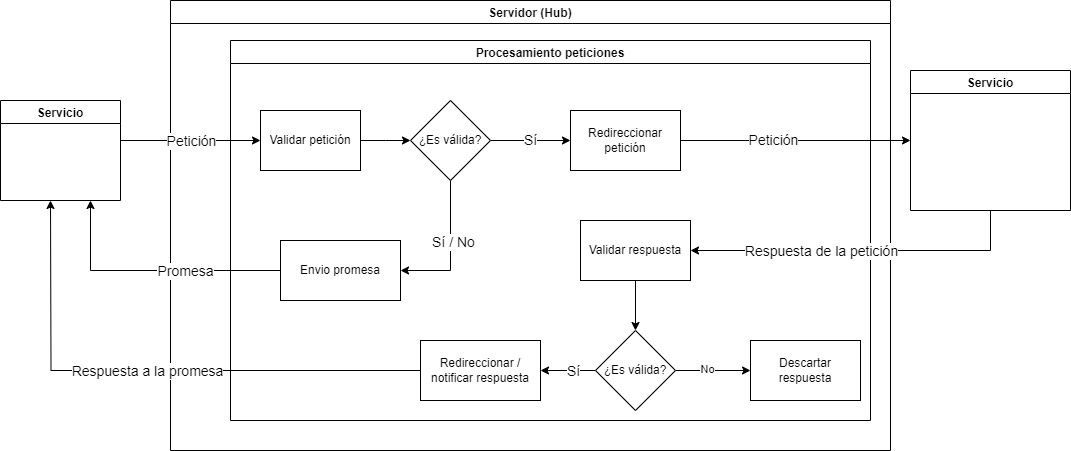
\includegraphics[width=\linewidth]{MVC/img/comunicacion.png}
    \caption{Comunicación entre elementos MVC y hub.}
    \label{fig:comuncacion mvc}
\end{figure}

Además, de la implementación comentada anteriormente, los \say{endpoints}/rutas del servidor se definen a través de un archivo de configuración JSON, el cual, mapea cada petición con los servicios, al igual que su respuestas pertinentes. Esto se puede ver en el siguiente ejemplo:

\begin{code}{\scriptsize}{json}
{
  "requestMap": [
    {
      "code": "SEND_GEOPOINTS",
      "services": ["MODEL", "CONTROLLER"]
    }
  ],
  "responseMap": [
    {
      "code": "LOAD_MAP",
      "services": ["VIEW"]
    },
  ],
}
\end{code}
